% Error Bounds
\section{Error Bounds}
Since the optimization function for each curve is not given access to 
derivative information, it is conceivable that it would not find the 
optimal value and instead converge to a local minimum.  However, the 
problem of escaping local minima is common to all optimization problems.  
The addition of the conditional that states: ``refine a segment if the 
refinement changes the length of the entire discretization by more than an 
epsilon'' was deliberately included to lessen the chance that a segment 
would not be refined when it was prudent to do so.  If the method succeeds 
in finding the global minimum for each segment, then the error bound will 
be on the order of the segment length.  However, when the method fails to 
do so, or chooses a local minimum instead, there is no formal way to 
express the error as a function of arclength-deficit--since there is no 
information about what the global minimum might be (without explicitly 
calculating the length of the curve/segment).  Therefore, the error can 
only be quantified for when the method has succeeded in finding the 
minimum for each segment.

Arclength-deficit is a single-value function on the curve.  The obvious 
problem with this single-valued function is that the actual arclength of 
the curve is never known and can therefore not be compared to the 
arclength of the segments.  How then can error be quantified? The error 
bounds could be detailed for unimodal pieces of the curve--those where the 
ALD function has one peak.  However, for segments that do not have a 
unimodal distribution of the ALD function on the local curve segment, the 
error estimation is not straightforward.  In fact, it is no longer 
possible to determine what the bound for the arclength-deficit error is.  
However, we can state some observations about the geometry related to 
these configurations:

Assume that the optimization function on a general segment found the global minimum, i.e. maximized the change in edge-length for the new combined segments, for the segment and corresponding curve piece.  With the given geometry, an ellipsoid can be formed with the endpoints of the segment, $F_1$ and $F_2$, as the foci and the semi-major and semi-minor axes are defined implicitly by the new segments connecting the new point with the endpoints of the current segment, $r_1$ and $r_2$.  ``An ellipse is a curve that is the locus of all points in the plane the sum of whose distances $r_1$ and $r_2$ from two fixed points $F_1$ and $F_2$ (the foci) separated by a distance of $2c$ is a given positive constant $2a$'' \cite{weissteine}.  With the above assumption and definition, the entirety of the curve represented by the segment must lie within the prolate spheroid  formed by the geometry below in \Cref{ref:EllipseGeometry}.

\begin{figure}[h!]
  \center{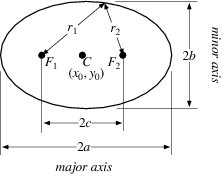
\includegraphics[height=1.5in]
    {Figures/EllipseGeometry.png}}
  \caption{\label{ref:EllipseGeometry} Caption}
\end{figure}

\begin{proof}
If the perimeter is maximized keeping $2c$ a constant, $(r_1 + r_2)$ is 
maximized \textit{because} $2c$ is a constant.  Maximizing $(r_1+r_2)$ 
maximizes a from the following relation with $2c$ being constant: $r_1 + 
r_2 = 2a$.  Combining the following relation, $b^2 = a^2 + c^2$, with the 
area of the ellipse, $A = \pi * a * b$, yields $A=\pi^{2}*a^{2}(a^{2} - 
c^2)$.  If $c$ is a constant and $a$ is maximized, then the maximal area 
is obtained from maximal $(r_1+r_2)$.  Which means the curve must be 
inside of the spheroid defined by the ellipse.  If the curve is not inside 
the spheroid then there is a point on the curve such that $(r_1+r_2)$ is 
larger and therefore the area is larger and therefore the volume is larger 
which means that $(r_1+r_2)$ was not maximized.
\end{proof}

Observe that there was no mention of the length of the curve inside of the 
spheroid, or the ruled area that the segment and curve could define.  
This is because there is no way this information can be known (without 
explicitly calculating the length of the curve/segment).  It is 
unfortunate that there is no way to quantify the discretization error of a 
curve except in terms of volume of the spheroids defined by each segment.  
This is non-intuitive, but no more specificity is possible.  The volumes 
would also be scale-dependent and offer no insight into how well the 
discretization approximates the curve -- without some context.
